%%
\bigheading{Connect Highways}
\authors{Gyula Horváth}{Gyula Horváth}{Gyula Horváth}
\heading{Naive solution}
Check for all pairs of points $a$ in Red and $b$ in Blue whether any segment of Red or Blue crosses the segment $\overline{(a,b)}$. The running time of this algorithm is $O(n_1 \, n_2 \, (m_1+m_2))$ where $n_1$ and $n_2$ are the number of points, $m_1$ and $m_2$ are the number of segments, respectively.
\heading{Linear time solution}
Let $a$ and $b$ be the points with least $y$-coordinates in Red and Blue networks, respectively:\\
\begin{center}
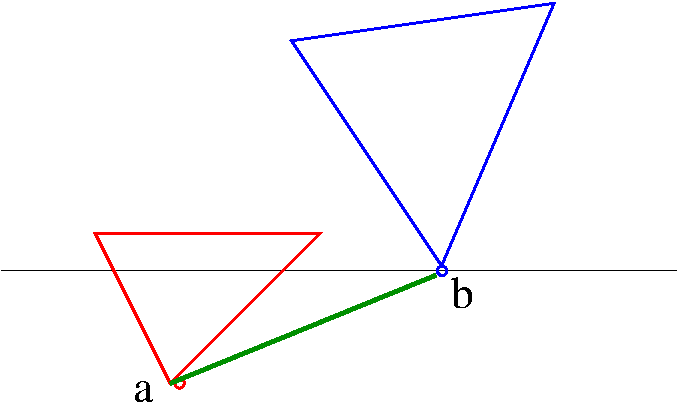
\includegraphics[height=4cm]{img/abra11.pdf}
\end{center}

$$a: ( \forall p \in Red)(a.y \leq p.y)$$
$$b: ( \forall p \in Blue)(b.y \leq p.y)$$
Without loss of the generality we assume that $a.y \leq b.y$.\\
We distinguish three cases.
\heading{Case 1: $a.y=b.y$}
\begin{center}
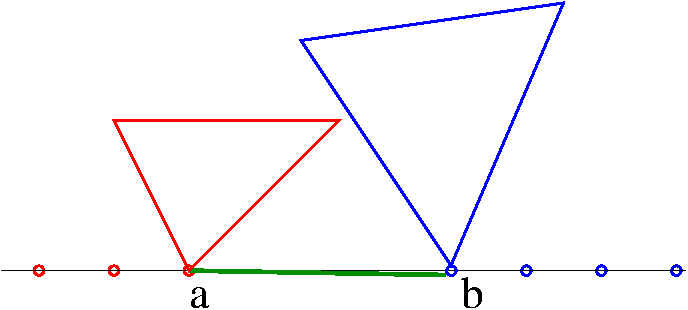
\includegraphics[height=4cm]{img/abra12.pdf}
\end{center}

In this case let $a$ and $b$ be the points such that there is no point between $a$ and $b$. In this case the pair $a \,b$  is a solution.
\heading{Case 2: $a.y<b.y$ and there is no segment crossing the segment $\overline{(a,b)}$}
In this case the pair $a \, b$ is a solution.\\
\begin{center}
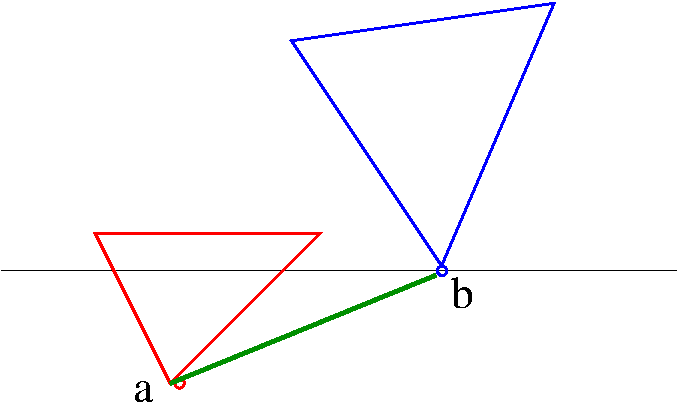
\includegraphics[height=4cm]{img/abra11.pdf}
\end{center}

\heading{Case 3: $a.y<b.y$ and there is a segment crossing the segment $\overline{(a,b)}$}
\begin{center}
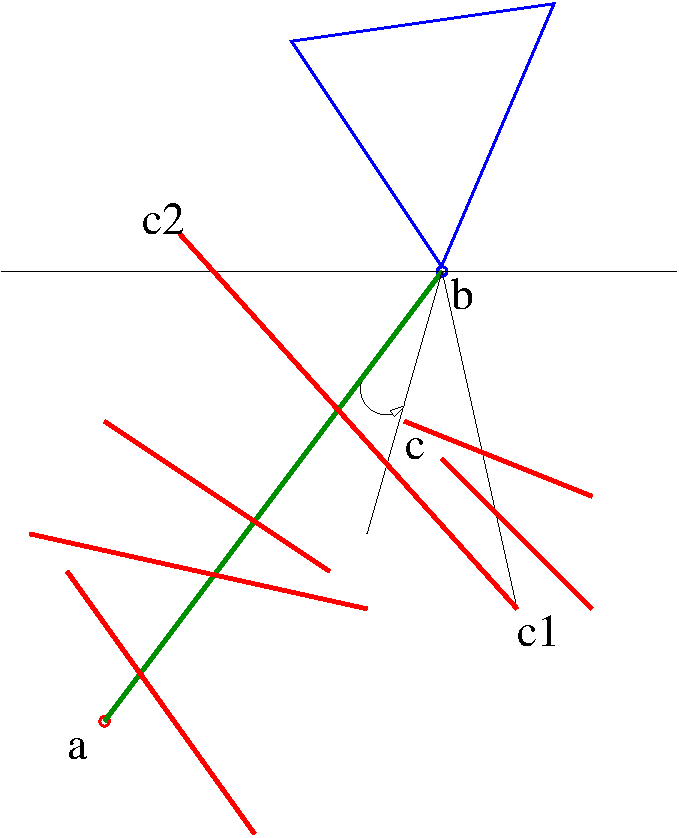
\includegraphics[height=6cm]{img/abra14.pdf}
\end{center}
Let $c1$ and $c2$ the endpoints of the  such that the intersection of the segment $(a,b)$ and the segment $(c1,c2)$ is closest to the point $b$. Assume that $c1.y<b.y$. Then the pair  $c1 \, b$ is a candidate solution. It is a solution if there is no segment crossing the segment $(c1, b)$. Otherwise take the point $c$ which is the endpoint of a crossing segment and there is no endpoint of crossing segment inside the triangle $(b,a,c)$. In this case the pair $c \, b$ is a solution.\\
In order to compute the segment $\overline{(c1,c2)}$ we define a linear ordering relation on the set of segments crossing the segment $\overline{(a,b)}$:\\
$$\overline{(p_1,p_2)} < \overline{(q_1,q_2)}$$
if and only if either of the case depicted in the  following figure hold.
\begin{center}
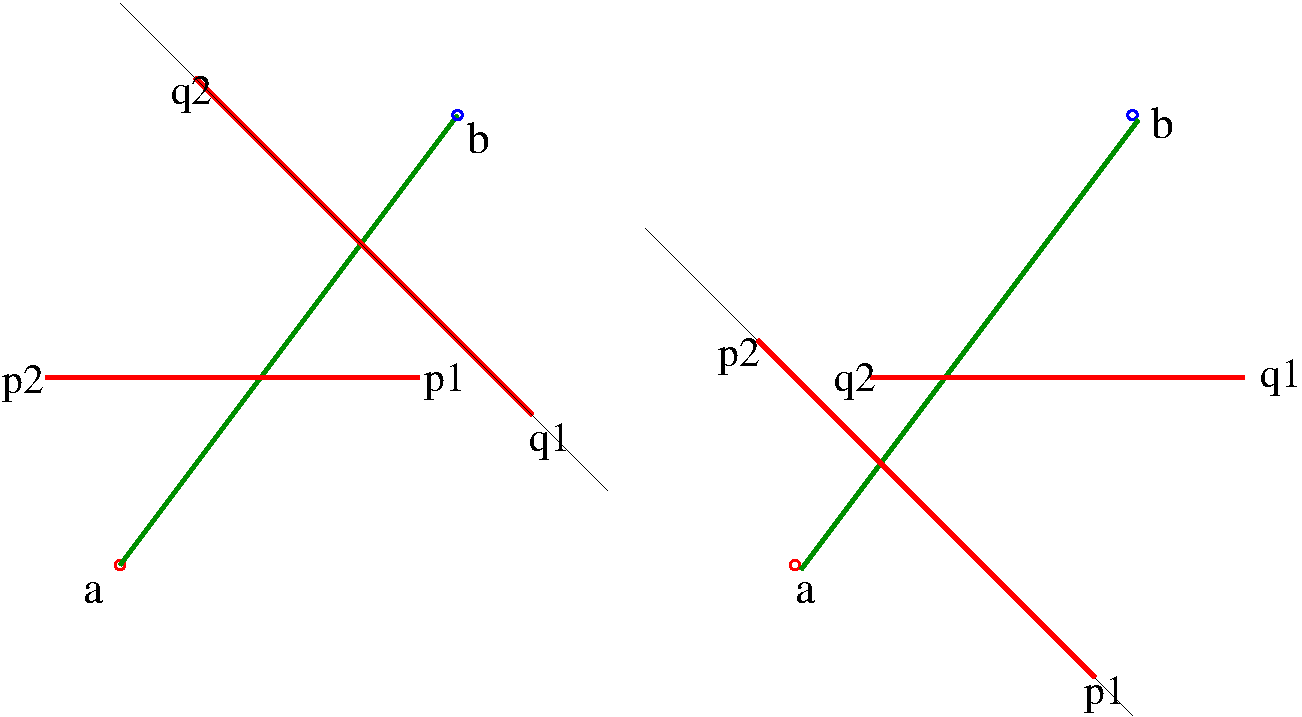
\includegraphics[height=4cm]{img/abra15.pdf}
\end{center}
It is clear, that segment $\overline{(c1,c2)}$ is the maximal element of the set of segments crossing the segment $\overline{(a,b)}$ according to the relation defined above. \\
For the implementation we need the following three basic geometry operations.\\
\lstlang{cpp}\begin{lstlisting}
int Turn(Point P0,Point P1,Point P2){
//Output:
//-1 iff P0-P1-P2 clockwise turn
// 0 iff P0,P1,P2 collinear
// 1 iff P0-P1-P2 counter-clockwise turn
   int64 crossp=(P1.x-P0.x)*(P2.y-P0.y)-(P2.x-P0.x)*(P1.y-P0.y);
   if (crossp<0)
      return -1;
   else if (crossp>0)
      return 1;
   else
      return 0;
}

bool Sless(Point p1, Point p2, Point q1, Point q2){
//Input: segment (p1,p2) and (q1,q2) crosses segment (a,b)
//Output: true iff intersection of (a,b) and (p1,p2) is closer to a then the intersection of (a,b) and (q1,q2)
   int pq1=Turn(p1,p2,q1);
   int pq2=Turn(p1,p2,q2);
   int qp1=Turn(q1,q2,p1);
   int qp2=Turn(q1,q2,p2);
   return pq1<=0 && pq2<=0 || qp1>=0 && qp2>=0;
}

bool Between(Point p1,Point p2, Point p3){
//Input: p1-p2-p3 collinear
//Output: true iff p3 is between p1 and p2
   return   (abs(p1.x-p3.x)<=abs(p2.x-p1.x)) &&
            (abs(p2.x-p3.x)<=abs(p2.x-p1.x)) &&
            (abs(p1.y-p3.y)<=abs(p2.y-p1.y)) &&
            (abs(p2.y-p3.y)<=abs(p2.y-p1.y)) ;
}
\end{lstlisting}

\emph{\textbf{Running time of the algorithm}}: $O(m_1+m_2)$ where $m_1$ and $m_2$ are the number of segments of Red and Blue networks, respectively.

